\chapter{Test Evidence}
\label{app:evidence}

This appendix indexes the raw evidence behind the bench results reported in Chapter~\ref{chap:method}. Every item is the unedited output of the test it names and is kept in the project repository, under \texttt{Report/evidence/} or \texttt{BenchTest/logs/}; Table~\ref{tab:evidence-index} gives each file. Figure~\ref{fig:live-dashboard} in Appendix~\ref{app:figures} and Figure~\ref{fig:recorded-session} in Chapter~\ref{chap:method} belong to the same record.

\begin{longtable}{|p{1.7cm}|p{3.6cm}|p{5.2cm}|p{3.6cm}|}
\caption{Index of test evidence.}
\label{tab:evidence-index}\\
\hline
\textbf{Date} & \textbf{Test} & \textbf{Result shown} & \textbf{File} \\ \hline
\endfirsthead
\hline
\textbf{Date} & \textbf{Test} & \textbf{Result shown} & \textbf{File} \\ \hline
\endhead
25 Sep 2026 & Recorded bench session, telemetry unit, 150\,s from power-up & 200\,Hz on both IMUs with no dropped samples; 149 fused windows, all from both sensors; five of five fusion self-tests passed; acquisition gaps of 25 to 30\,ms every 12\,s & \texttt{BenchTest/logs/ 2026-09-25\_bench\_fusion\_shake.log} \\ \hline
25 Sep 2026 & The same log replayed through the bench console (Figure~\ref{fig:console-replay}) & Every subsystem's state at the end of the session, and the vibration and disagreement traces for the whole recording & \texttt{Report/evidence/ 2026-09-25\_bench\_console\_replay.png} \\ \hline
28 Sep 2026 & Hazard detector, first run on live camera frames & 430 frames in 60.1\,s (7.2\,fps); a person in view logged as ``motorcycle'', which exposed the label-offset fault & \texttt{Report/evidence/ 2026-09-28\_camera\_run1\_label\_bug.txt} \\ \hline
28 Sep 2026 & Hazard detector after the label and colour fixes & 419 frames in 60.1\,s (7.0\,fps); person detected at confidence 0.50 to 0.73; 16 alert activations in 47\,s for one person in view, which led to clear-side hysteresis & \texttt{Report/evidence/ 2026-09-28\_camera\_run2\_after\_fixes.txt} \\ \hline
29 Sep 2026 & Firmware v0.5.0 on the telemetry unit: commands, flash-write stall test, MQTT reconnect & With logging on, 33 to 40\,ms gaps on both IMUs every 10\,s; with logging off, worst gap 5.9\,ms; no dropped samples; 47 MQTT publishes with no failures; reconnect in 0.4\,s & \texttt{BenchTest/logs/ 2026-09-29\_v050\_bench\_test.log} \\ \hline
29 Sep 2026 & GNSS outdoor fix on a rooftop, firmware v0.5.0, raw replies requested every 15\,s & 3D fix after 51\,s; 17-field reply with decimal degrees; old parser read satellite counts as the position; well-formed replies 2.4 and 5.5\,m from the phone's position; replies garbled by the competing query & \texttt{BenchTest/logs/ 2026-09-29\_gnss\_rooftop.log} \\ \hline
30 Sep 2026 & GNSS outdoor fix with the corrected parser (v0.5.2), raw replies printed by the firmware & 3D fix after 105\,s from a cold start; 23 to 25 satellites; over 104 fixes, median 2.7\,m and 95\% within 11.0\,m of the phone's position & \texttt{BenchTest/logs/ 2026-09-30\_gnss\_rooftop\_v052.log} \\ \hline
30 Sep 2026 & MQTT recovery from a 60\,s radio-off period (\texttt{AT+CFUN=4}, then \texttt{AT+CFUN=1}), v0.5.0 and v0.5.3 & Loss detected in 0.8 to 20.7\,s; retries at 30 and 60\,s; reconnect 36\,s after the radio returned in v0.5.0, about 5\,s in v0.5.3; no failed publishes afterwards & \texttt{BenchTest/logs/ 2026-09-30\_signal\_loss\_test.log}, \texttt{..\_v053.log} \\ \hline
30 Sep 2026 & Sync-pulse edges logged on the Pi (GPIO17, kernel timestamps), two 60\,s runs & Run 1: 16\,s burst of spurious edges, consistent with a disturbed contact; run 2: 121 edges, median interval 500.06\,ms, range 499.72 to 500.41\,ms & \texttt{BenchTest/logs/ 2026-09-30\_sync\_edges\_run1\_noisy.csv}, \texttt{..\_run2.csv} \ \hline
30 Sep 2026 & Camera detector latency on the Pi, three 60\,s runs (4 threads, 4 threads with live view, 1 thread) & Median 102, 105 and 186\,ms from sensor readout to result; 19.5, 17.3 and 7.0 frames per second; no throttling & \texttt{BenchTest/logs/ 2026-09-30\_c4\_latency/} \ \hline
\end{longtable}

\begin{figure}[htbp]
\centering
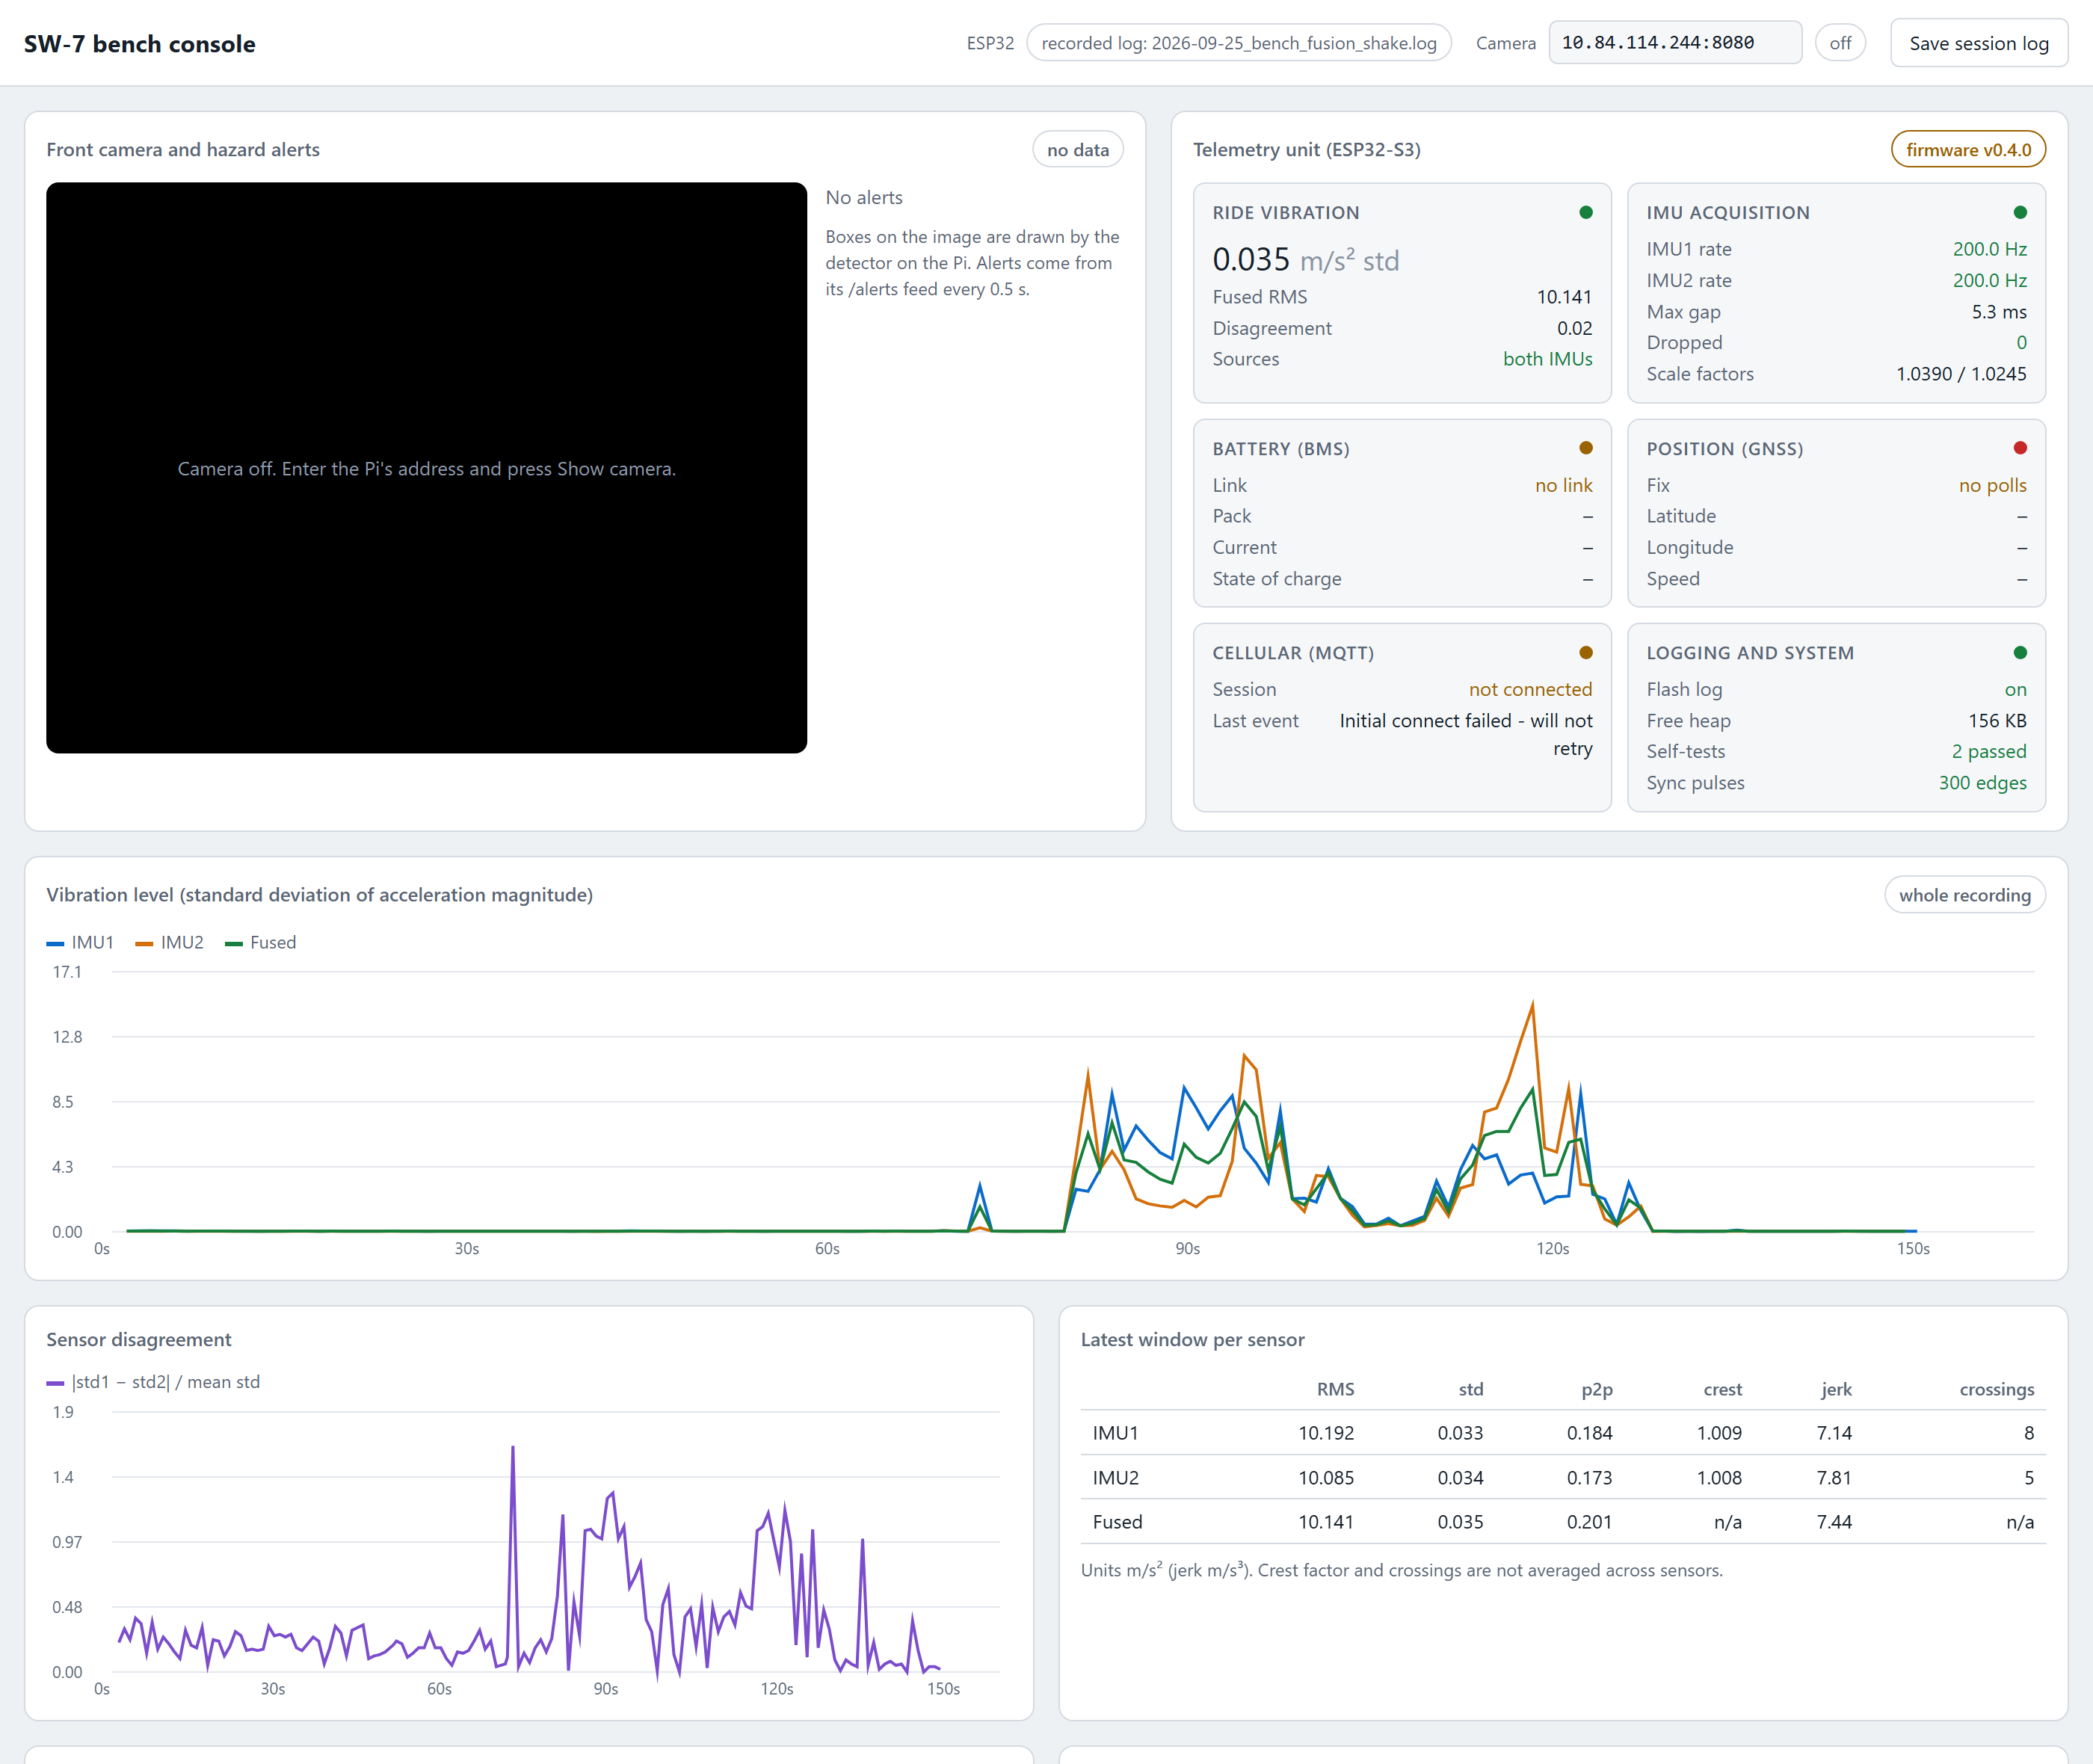
\includegraphics[width=\textwidth]{evidence/2026-09-25_bench_console_replay.png}
\caption{The recorded bench session of 25 September 2026 replayed through the bench console, which parses the telemetry unit's serial output. Only recorded data is shown; the camera panel is off because the camera was not part of this session.}
\label{fig:console-replay}
\end{figure}

The two detector runs end with the following lines, copied from the Raspberry Pi terminal. Before the fixes, every alert carried the wrong class:

\begin{verbatim}
Stopped. 430 frames in 60.1s (7.2 fps average).
{"class": "motorcycle", "distance_band": "immediate", "confidence": 0.66,
 "timestamp": "2026-09-28T11:58:32", "alert_status": "active"}
\end{verbatim}

After the fixes, the class is correct, and the log shows the alert clearing and re-activating within a few seconds while the same person stayed in view:

\begin{verbatim}
[14:31:28] person band=immediate conf=0.59 streak=3/3
  -> ALERT logged: person (immediate)
Stopped. 419 frames in 60.1s (7.0 fps average).
{"class": "person", "distance_band": "immediate", "confidence": 0.59,
 "timestamp": "2026-09-28T14:31:28", "alert_status": "active"}
{"class": "person", "distance_band": null, "confidence": 0.0,
 "timestamp": "2026-09-28T14:31:30", "alert_status": "cleared"}
{"class": "person", "distance_band": "immediate", "confidence": 0.59,
 "timestamp": "2026-09-28T14:31:31", "alert_status": "active"}
\end{verbatim}
